%Author: Stanislav Letaši xletas00@vutbr.cz
\documentclass[a4paper,11pt]{article}
\usepackage[slovak]{babel}
\usepackage[a4paper, total={170mm, 240mm}, top=2cm, left=2cm]{geometry}
\usepackage[utf8]{inputenc}
\usepackage[IL2]{fontenc}
\usepackage{times}
\usepackage[hidelinks]{hyperref}
\usepackage{graphicx}
\usepackage{booktabs}
\usepackage{epstopdf}
\usepackage[htt]{hyphenat}
\usepackage{amsmath}
\usepackage{float}
\usepackage{indentfirst}
\usepackage{array}
\usepackage{enumitem}
\usepackage{bm}

\begin{document}
\begin{center}
\Huge
\textsc{Vysoké učení technické v~Brně\\
}Fakulta informačních technologií\\
\vspace{\stretch{0.382}}
\Huge Projektová dokumentácia \\
\LARGE Implementácia prekladača jazyka IFJ23 \\
\Large Tím xkruli03, varianta TRP-izp\\
\vspace{\stretch{0.309}}

\Large 

\vspace{\stretch{0.309}}

\end{center}
{\Large \today \hfill
\begin{tabular}{l r c r}
            &Boris Hatala	      &(xhatal02)	&25\%	\\
            &František Holáň	  &(xholan13)	&25\%	\\
        	&Michal Krulich	      &(xkruli03)	&25\%	\\ 
			&Stanislav Letaši	  &(xletas00)	&25\%	\\
\end{tabular}}
\thispagestyle{empty}

\newpage

\tableofcontents

\newpage

\section{Úvod}
Táto dokumentácia obsahuje popis implementácie interpretu jazyka IFJ23, čo je zjednodušená verzia jazyka Swift 5. Swift 5 je staticky typovaný jazyk, ktorý kombinuje prvky objektovo orientovaného, funkcionálneho a imperatívneho programovania.

Nami zvolená varianta je TRP-izp, čo znamená, že tabuľka symbolov je implementovaná ako tabuľka s rozptýlenými položkami s implicitným zreťazením položiek.

\subsection{Štruktúra zdrojových súborov}

\begin{itemize}

    \item \texttt{decode.h decode.c} - Konvertuje reťazec napísaný v zdrojovom jazyku na reťazec pre IFJcode23
    
    \item \texttt{dll.h dll.c} - Implementácia dvojsmerného zoznamu pre generované inštrukcie
    
    \item \texttt{exp.h exp.c} - Precedenčná analýza výrazov s generovaním cieľového kódu
    
    \item \texttt{generator.h generator.c} - Generátor cieľového kódu
    
    \item \texttt{logErr.h logErr.c} - Pomocné funkcie pre hlásenie chýb 
    prekladu kódu či samotného prekladača
    
    \item \texttt{main.c} - Hlavné telo prekladača 
    
    \item \texttt{parser.h parser.c} - Syntaktický a sémantický anayzátor
    
    \item \texttt{scanner.h scanner.c} - Lexikálny analyzátor
    
    \item \texttt{strR.h strR.c} - Implementácia reťazca s automatickou 
    realokáciou veľkosti
    
    \item \texttt{symtable.h symtable.c} - Tabuľka symbolov
    
\end{itemize}
\section{Implementácia}

\subsection{Skener}
Hlavným cieľom implementácie lexikálnej analýzy je funkcia \texttt{getToken()}. Táto funkcia číta jednotlivé znaky zo štandardného vstupu a má za úlohu rozpoznať lexémy zdrojového jazyka a vrátiť príslušné tokeny. Token je reprezentovaný štruktúrou, v ktorej je uložený typ tokenu (rozpoznáva sa celkom 42 rôznych typov tokenov), reťazec načítaného lexému, riadok a stĺpec prečítaného lexému.

\subsubsection{Konečný automat}
Celý lexikálny analyzátor je implementovaný ako deterministický konečný automat obsahujúci ukončujúce a neukončujúce stavy. Tento automat bol naprogramovaný ako jeden \texttt{switch}, kde každé náveštie \texttt{case} reprezentuje jeden stav automatu. Okrem hlavného \texttt{switch} statementu vo funkcii \texttt{getToken()}, je tiež implementovaný podautomat v pomocnej funkcii, ktorý spracováva escape sekvencie v reťazcoch (za účelom sprehľadnenia kódu).

Počas čítania znakov zdrojového kódu zo štandardného vstupu sa prechádza medzi jednotlivými stavmi. Pokiaľ sa automat nachádza v ukončujúcom stave a ďalší načítaný znak už nezodpovedá tokenu, ktorý je reprezentovaný aktuálnym stavom, je vrátený príslušný token. Ak je načítaný znak ktorý nesúhlasí so žiadnym znakom, ktorý by jazyk IFJ23 povoľoval, je vrátený token s hodnotou \texttt{0}, značiaci chybu počas lexikálnej analýzy. Rovnako tak sa deje, ak sa nachádza automat v neukončujúcom stave a na vstupe je znak, po prečítaní ktorého by výsledná sekvencia načítaných znakov nezodpovedala žiadnemu typu tokenu.

Špecifická je situácia týkajúca sa rozpoznania identifikátorov a kľúčových slov. Automat nezahŕňa žiadny stav pre kľúčové slová, ale iba stav pre identifikátor. Ak nastane ukončenie čítania znakov v stave identifikátora, skontroluje sa, či nie je načítaný reťazec (uložený vždy v príslušnom atribúte tokenu) zhodný s niektorým z kľúčových slov jazyka IFJ23. Takto sa rozpozná, či ide o identifikátor alebo o kľúčové slovo.

Okrem funkcie \texttt{getToken()} je tiež implementovaná špeciálna funkcia \texttt{storeToken(tkn)}, ktorá pri zavolaní uloží token \texttt{tkn} do globálnej premennej \texttt{storage}.

\subsection{StrR}
Slúži na uchovanie reťazcov predom neznámej dĺžky. Tento reťazec automaticky
realokuje svoju veľkosť vzhľadom na dĺžku vstupného reťazca. Je používaný v
každej časti prekladača.

Okrem základných operácií ako inicializácia a deštrukcia reťazca sú implementované aj ďalšie
funkcie. Pridanie znaku na koniec dynamického reťazca, zaplnenie reťazca s obsahom
klasického reťazca jazyku C, spojenie dvoch dynamických reťazcov alebo spojenie
dynamického reťazca s reťazcom jazyka C a vrátenie ukazateľa na dáta v dynamickom reťazci.

\subsection{DLL}
Na uchovávanie generovaného cieľového kódu je využívaný dvojsmerne viazaný zoznam reťazcov. Pri vkladaní nového reťazca do zoznamu je vytvorený nový prvok zoznamu \texttt{DLLstr\textunderscore element} a alokovaná nová kópia reťazca, ktorá je uložená do tohto zoznamu. Dvojsmernosť zoznamu je hlavne využívaná pri generovaní kódu deklarácii premenných nachádzajúcich sa vo vnútri cyklu, kde musia byť tieto inštrukcie zapísané pred samotný cyklus. Zároveň je táto dátová štruktúra používaná pre uchovávanie názvov a identifikátorov parametrov funkcií.

\subsection{Tabuľka symbolov}
Tabuľka symbolov je v prekladači implementovaná pomocou zreťazených tabuliek s rozptýlenými položkami s implicitným zreťazením položiek, pričom tieto jednotlivé tabuľky/bloky sú usporiadané vo forme zoznamu. Každý blok tabuľky symbolov \texttt{TSBlock\textunderscore T} obsahuje pole ukazateľov na prvky \texttt{TSData\textunderscore T}, ktoré sú dátovými štruktúrami reprezentujúcimi informácie o premenných alebo funkciach. Každý prvok obsahuje informácie ako názov identifikátora/funkcie, typ (napríklad \texttt{i} pre Integer, \texttt{F} pre funkciu), informáciu o inicializácii či modifikovateľnosti premennej, prípadne signatúru funkcie \texttt{func\textunderscore sig\textunderscore T}.

Bloky tabuľky symbolov sú dvojsmerne zreťazené v zozname, kde prvý blok obsahuje informácie o globálnych premenných a funkciách. Metódy nad tabuľkou umožňujú pridávať a odstraňovať ďalšie (lokálne) bloky na konci zoznamu, ktorých význam spočíva v simulácii zanorovania a prekrývania premenných.

Hľadanie a vkladanie symbolov v tabuľke je realizované pomocou dvoch rozptylovacích funkcií, kde prvá (djb2\footnote{\url{http://www.cse.yorku.ca/~oz/hash.html}}) určuje počiatočný index a druhá (upravený djb2) veľkosť kroku pri hľadaní ďalšieho synonyma. Implementované verejné metódy umožňujú vyhľadávať či vkladať priamo do globálneho alebo posledného lokálneho bloku.


\subsection{Parser}
Najväčšiu časť prekladača tvorí syntaktický analyzátor (parser), ktorý zároveň vykonáva syntaktickú analýzu, sémantickú analýzu a generovanie cieľového kódu. Parser komunikuje so všetkými podčasťami prekladača a to: získavanie tokenov od skenera, sémantické kontroly s údajmi ukladanými do tabuľky symbolov a generovanie cieľového kódu (\texttt{generator.h}).

Syntaktická analýza programu prebieha dvomi rôznymi technikami, ktoré si medzi sebou vymieňajú riadenie. Na začiatku behu prekladača sa spracúva program technikou \textit{top-down} analýzy a pri nájdení začiatku výrazu je riadenie odovzdané \textit{bottom-up} analýze, ktorá končí po zostavení najdlhšieho možného výrazu, prípadne zistení syntaktickej či sémantickej chyby vo vnútri výrazu, a odovzdáva riadenie naspäť. Samotná \textit{top-down} analýza je spustená v súbore \texttt{main.c} v hlavnom cykle, ktorý spracúva jednotlivé príkazy hlavného tela programu a definície funkcií, a končí načítaním konca programu.


\subsubsection{Rekurzívny zostup}
Rekurzívny zostup sa vykonáva pomocou funkcií definovaných v \texttt{parser.c}, kde každej tejto funkcii náleží jedno pravidlo definovanej LL-gramatiky a nasledujúci zostup je rozhodnutý podľa LL-tabuľky. Špeciálny prístup sa uplatňuje pri volaniach funkcií, keďže rozlíšenie beznávratového volania funkcie od priradenia a volania funkcie od výrazu nie je na základe jedného tokenu možné. V takom prípade je prečítaný ešte jeden token a v prípade nepotvrdenia volania funkcie je tento token vrátený naspäť skeneru.

	Návratová hodnota všetkých funkcií rekurzívneho zostupu je v prípade správneho programu \texttt{0} alebo v prípade nájdenia chyby rovná číslu chyby, pričom chybová hláška je vypísaná v najnižšom rekurzívnom zanorení. Niektoré z týchto funkcií obsahujú zvláštne parametre, ktoré slúžia pre ďalšie sémantické kontroly a generovanie kódu. Pomocné dáta ako aktuálne načítaný token, ukazateľ na tabuľku symbolov, názov aktuálne spracovávanej funkcie či cyklu, alebo zoznam premenných definovaných v cykle sú používané naprieč všetkými funkciami \textit{top-down} analýzy a preto sú deklarované ako globálne premenné.
	
 Počas rekurzívneho zostupu prebieha aj sémantická analýza kódu, pričom je často využívaná tabuľka symbolov, a to pre kontrolu deklarovaných funkcií a premenných, ich signatúr/dátových typov, informácii, či boli definované/inicializované ale aj simuláciu blokov rozsahu a vnorení.

\subsubsection{Precedenčná analýza}
Analýza výrazov začína syntaktickou kontrolou. Spracovávaný je každý token výrazu, pričom je uchovávaný aj typ predošlého tokenu. Syntaktická analýza nie je implementovaná ako konečný automat, ale skôr ako \uv{filter} syntaktických chýb. Počas syntaktickej analýzy prebieha aj konverzia pôvodného výrazu do postfixovej formy, pričom sa z tabuľky symbolov získavajú ďalšie informácie o premenných a kontroluje sa ich stav deklarácie a inicializácie. Syntaktická analýza úspešne končí, ak spracovávaný token nemôže patriť do výrazu, a doteraz spracovaný výraz je syntakticky správny.

Počas sémantickej analýzy sú spracovávané tokeny z postfixového výrazu, prebieha generácia kódu a na pomocnom zásobníku tokenov je vytváraný finálny dátový typ výrazu, ktorý bude po skončení predaný naspäť pre \textit{top-down} analýzu. Sémantická analýza taktiež vykonáva konverziu int konštánt na double, ak je to potrebné, a pre \textit{top-down} analýzu vracia späť informáciu, či je finálny výraz možné implicitne prekonvertovať na double.

\subsection{Generovanie cieľového kódu}
Cieľové inštrukcie sú generované použitím pomocných funkcií v rozhraní \texttt{generator.h}, ktoré sú v rekurzívnom zostupe volané popri syntaktickej analýze a v precedenčnej analýze popri sémantickej analýze. Vygenerovaný kód je uchovávaný v dvoch zoznamoch, kde \texttt{code\textunderscore fn} uchováva inštrukcie užívateľom definovaných funkcií a \texttt{code\textunderscore main} prestavuje hlavné telo programu. 

Výsledný vygenerovaný kód je vytlačený na štandardný výstup pomocou funkcie \texttt{printOutCompiledCode()}. Táto funkcia pridá potrebnú hlavičku .IFJcode23, tri špeciálne pomocné globálne premenné, inštrkuciu skoku do hlávneho programu a následne vytlačí obsah \texttt{code\textunderscore fn} a \texttt{code\textunderscore main} spolu s náveštím na hlavné telo programu.

\subsubsection{Názvy premenných a náveští}
Pretože nie je možné v interprete medzikódu IFJcode23 používať dočasný rámec a zásobník lokálnych rámcov ako spôsob zanorovania a prekrývania premenných, tak je každému identifikátoru premennej pomocou funkcie \texttt{genUniqVar} pridané unikátne číslo, ktoré zaisťuje rozlíšenie od možných prekrytých premenných. Podobný prístup priraďovania unikátnych čísel je zavedený aj pri náveštiach konštrukcií \texttt{while}, \texttt{if} a operátorov \texttt{??}, kedy je používaná funkcia \texttt{genUniqLabel}.

\subsubsection{Definície funkcií a ich volanie}
Definície užívateľských funkcií začínajú náveštím s názvom funkcie, vytvorením vlastného lokálneho rámca uloženého na vrchol zásobníka rámcov a spracovaním argumentov, ktoré boli predané cez klasický zásobník. Nasleduje samotný kód funkcie, a vždy končí inštrukciou \texttt{RETURN}. Ak funkcia vracia nejakú hodnotu, tak táto hodnota je vložená na vrchol zásobníka pred samotným \texttt{RETURN}.

Volanie funkcie začína vkladaním argumentov od posledného k prvému (prvý argument bude na vrchole). Následne sa zavolá daná funkcia pomocou inštrukcie \texttt{CALL} a zahodí sa lokálny rámec vytvorený funkciou a prípadne sa získa návratová hodnota zo zásobníka alebo sa zásobník vyprázdni pomocou \texttt{CLEARS}.
Pretože premenné deklarované v hlavnom tele programu sa nachádzajú v globálnom rámci a každé volanie funkcie vytvára nový lokálny rámec na zásobniku rámcov, tak je zabránené akejkoľvek kolízii pri rekurzívnom volaní. 

 \subsubsection{Vstavané funkcie}
 Väčšina vstavaných funkcií je implementovaných pomocou jednej alebo dvoch inštrukcií a nie je preto potrebné pri ich volaní generovať inštrukciu \texttt{CALL} či vytvárať nový lokálny rámec. Výnimku tvorí vstavaná funkcia \texttt{substring}, ktorá je natoľko komplexná, že jej vlastný súbor inštrukcií bude dodatočne vložený k bežným užívateľom definovaným funkciám, pokiaľ bola v priebehu programu aspoň raz volaná.






\section{Vývojový cyklus}
\subsection{Práca v tíme}
Prácu na projekte sme zahájili úvodnou schôdzou na začiatku októbra. Na tejto schôdzi sme si rozdelili hlavné časti projektu medzi jednotlivých členov tímu, pripravili sme si približný časový harmonogram (stanovili sme si termíny, do kedy chceme mať hotové konkrétne časti projektu) a dohodli sme sa na ďalších záležitostiach potrebných na prácu. Na konkrétnych celkoch sme pracovali väčšinou jednotlivo.

\subsection{Vývojové prostredie}
Dohodli sme sa, že pri vývoji budeme používať prostredie Visual Studio Code. S týmto vývojovým prostredím sme mali všetci skúsenosti, preto sme túto voľbu považovali za najprijateľnejšiu. Výhodou pri vývoji v tomto prostredí bolo okrem iného prepojenie s GitHub serverom, čo viedlo k jednoduchšej práci s naším repozitárom.

\subsection{Repozitár}
Na správu súborov sme používali systém Git, pričom ako vzdialený repozitár sme využili GitHub.

\subsection{Komunikácia v tíme}
Komunikácia prebiehala hlavne prostredníctvom serveru Discord. Poväčšine sme komunikovali v skupinovom chate, aby všetci členovia tímu boli informovaní o vývoji.
Nevyhnutnou súčasťou boli aj osobné stretnutia, ktoré sme organizovali vždy pred začiatkom práce na rozsiahlejšom celku, aby sme vyriešili ďalší postup.
\newpage
\subsection{Rozdelenie práce medzi členov tímu}
Prácu v tíme sme sa snažili rozdeliť čo najrovnomernejšie. Dohodli sme sa, že každý člen tímu dostane percentuálne hodnotenie 25\%. Tabuľka nižšie zobrazuje rozdelenie práce medzi členov tímu.

\medskip

\begin{tabular}{lp{11.9cm}}
	\textbf{Boris Hatala} & tabuľka symbolov, pomocné funkcie pre generovanie kódu, funkcie pre prácu s řeťazcami, dokumentácia \\
	\textbf{František Holáň}  & lexikálna analýza, pomocné funkcie pre generovanie kódu, dokumentácia \\
	\textbf{Michal Krulich} & vedenie tímu, organizácia práce, syntaktická a sémantická analýza – \textit{top-down}, testovanie, generovanie kódu, dokumentácia \\
	\textbf{Stanislav Letaši} & syntaktická a sémantická analýza – \textit{bottom-up}, finálne zpracovanie dokumentácie \\
\end{tabular}


\medskip
\newpage
\appendix
\section{Prílohy}
\subsection{Pravidlá bezkontextovej gramatiky používanej parserom}

\begin{enumerate}[itemsep=-0.2ex]
    \small
    \item $<$STAT$>$ $\rightarrow$ $\epsilon$
    \item $<$STAT$>$ $\rightarrow$ let id $<$DEF\_VAR$>$ $<$STAT$>$
    \item $<$STAT$>$ $\rightarrow$ var id $<$DEF\_VAR$>$ $<$STAT$>$
    \item $<$DEF\_VAR$>$ $\rightarrow$ : $<$TYPE$>$ $<$INIT\_VAL$>$
    \item $<$DEF\_VAR$>$ $\rightarrow$ = $<$ASSIGN$>$
    \item $<$INIT\_VAL$>$ $\rightarrow$ = $<$ASSIGN$>$
    \item $<$INIT\_VAL$>$ $\rightarrow$ $\epsilon$
    \item $<$ASSIGN$>$ $\rightarrow$ exp
    \item $<$ASSIGN$>$ $\rightarrow$ id ( $<$PAR\_LIST$>$ )
    \item $<$STAT$>$ $\rightarrow$ id = $<$ASSIGN$>$ $<$STAT$>$
    \item $<$STAT$>$ $\rightarrow$ \{ $<$STAT$>$ \} $<$STAT$>$
    \item $<$STAT$>$ $\rightarrow$ id ( $<$PAR\_LIST$>$ ) $<$STAT$>$
    \item $<$PAR\_LIST$>$ $\rightarrow$ id : term $<$PAR\_IN\_NEXT$>$
    \item $<$PAR\_LIST$>$ $\rightarrow$ term $<$PAR\_IN\_NEXT$>$
    \item $<$PAR\_LIST$>$ $\rightarrow$ $\epsilon$
    \item $<$PAR\_IN\_NEXT$>$ $\rightarrow$ , $<$PAR\_IN$>$ $<$PAR\_IN\_NEXT$>$
    \item $<$PAR\_IN\_NEXT$>$ $\rightarrow$ $\epsilon$
    \item $<$PAR\_IN$>$ $\rightarrow$ id : term
    \item $<$PAR\_IN$>$ $\rightarrow$ term
    \item $<$STAT$>$ $\rightarrow$ func id ( $<$FN\_SIG$>$ ) $<$FN\_RET\_TYPE$>$ \{ $<$STAT$>$ \} $<$STAT$>$
    \item $<$FN\_SIG$>$ $\rightarrow$ id id : $<$TYPE$>$ $<$FN\_PAR\_NEXT$>$
    \item $<$FN\_SIG$>$ $\rightarrow$ \_ id : $<$TYPE$>$ $<$FN\_PAR\_NEXT$>$
    \item $<$FN\_SIG$>$ $\rightarrow$ $\epsilon$
    \item $<$FN\_PAR\_NEXT$>$ $\rightarrow$ , $<$FN\_PAR$>$ $<$FN\_PAR\_NEXT$>$
    \item $<$FN\_PAR\_NEXT$>$ $\rightarrow$ $\epsilon$
    \item $<$FN\_PAR$>$ $\rightarrow$ id id : $<$TYPE$>$
    \item $<$FN\_PAR$>$ $\rightarrow$ \_ id : $<$TYPE$>$
    \item $<$FN\_PAR$>$ $\rightarrow$ id \_ : $<$TYPE$>$
    \item $<$FN\_PAR$>$ $\rightarrow$ \_ \_ : $<$TYPE$>$
    \item $<$FN\_RET\_TYPE$>$ $\rightarrow$ $->$ $<$TYPE$>$
    \item $<$FN\_RET\_TYPE$>$ $\rightarrow$ $\epsilon$
    \item $<$STAT$>$ $\rightarrow$ return $<$RET\_VAL$>$ $<$STAT$>$
    \item $<$RET\_VAL$>$ $\rightarrow$ exp
    \item $<$RET\_VAL$>$ $\rightarrow$ $\epsilon$
    \item $<$STAT$>$ $\rightarrow$ if $<$COND$>$ \{ $<$STAT$>$ \} else \{ $<$STAT$>$ \} $<$STAT$>$
    \item $<$COND$>$ $\rightarrow$ exp
    \item $<$COND$>$ $\rightarrow$ let id
    \item $<$STAT$>$ $\rightarrow$ while exp \{ $<$STAT$>$ \} $<$STAT$>$
    \item $<$TYPE$>$ $\rightarrow$ Integer $<$QUESTMARK$>$
    \item $<$TYPE$>$ $\rightarrow$ Double $<$QUESTMARK$>$
    \item $<$TYPE$>$ $\rightarrow$ String $<$QUESTMARK$>$
    \item $<$QUESTMARK$>$ $\rightarrow$ ?
    \item $<$QUESTMARK$>$ $\rightarrow$ $\epsilon$
\end{enumerate}

\subsection{Precedenčná tabuľka}
\begin{table}[htbp]
    \centering
    \begin{tabular}{|c||*{8}{c|}}
        \hline
        \textbf{} & \textbf{!} & \textbf{* /} & \textbf{+ -} & \textbf{id} & \textbf{rel} & \textbf{??} & \textbf{(} & \textbf{)} \\
        \hline\hline
        \textbf{!} & & $>$ & $>$ & & $>$ & $>$ &  & $>$ \\
        \hline
        \textbf{* /} & $<$ & $>$ & $>$ & $<$ & $>$ & $>$ & $<$ & $>$ \\
        \hline
        \textbf{+ -} & $<$ & $<$ & $>$ & $<$ & $>$ & $>$ & $<$ & $>$ \\
        \hline
        \textbf{id} & $>$ & $>$ & $>$ & & $>$ & $>$ & & $>$ \\
        \hline
        \textbf{rel} & $<$ & $<$ & $<$ & $<$ &  & $>$ & $<$ & $>$ \\
        \hline
        \textbf{??} & $<$ & $<$ & $<$ & $<$ & $<$ & $<$ & $<$ & $>$ \\
        \hline
        \textbf{(} & $<$ & $<$ & $<$ & $<$ & $<$ & $<$ & $<$ & = \\
        \hline
        \textbf{)} & $>$ & $>$ & $>$ &  & $>$ & $>$ &  & $>$ \\
        \hline
    \end{tabular}
    \caption{\textbf{id} - identifikátor, \textbf{rel} - relačné operátory ($$==$$, $<$$=$, \dots)}
\end{table}


\subsection{LL tabuľka}
\begin{table}[htbp]

\scriptsize
\setlength{\tabcolsep}{0.51\tabcolsep}
\renewcommand{\arraystretch}{1.2}
\begin{tabular}{|c||c|c|c|c|c|c|c|c|c|c|c|c|c|c|c|c|c|c|c|c|}

\hline
              & \multicolumn{1}{c|}{\textbf{id}}     & \multicolumn{1}{c|}{\textbf{:}} & \multicolumn{1}{c|}{\textbf{=}} & \multicolumn{1}{c|}{\textbf{\{}} & \multicolumn{1}{c|}{\textbf{term}} & \multicolumn{1}{c|}{\textbf{return}} & \multicolumn{1}{c|}{\textbf{Integer}} & \multicolumn{1}{c|}{\textbf{Double}} & \multicolumn{1}{c|}{\textbf{String}} & \multicolumn{1}{c|}{\textbf{exp}} & \multicolumn{1}{c|}{\textbf{func}} & \multicolumn{1}{c|}{\textbf{if}} & \multicolumn{1}{c|}{\textbf{let}} & \multicolumn{1}{c|}{\textbf{var}} & \multicolumn{1}{c|}{\textbf{while}} & \multicolumn{1}{c|}{\textbf{?}}  & \multicolumn{1}{c|}{\textbf{\textunderscore}}     & \multicolumn{1}{c|}{\textbf{,}}  & \multicolumn{1}{c|}{$\bm{-\!>}$} & \textbf{\$}                     \\ 
\hline\hline
\textbf{$<$STAT$>$}          & \multicolumn{1}{c|}{10, 12} &                        &                        & \multicolumn{1}{c|}{11} &                           & \multicolumn{1}{c|}{30}     &                              &                             &                             &                          & \multicolumn{1}{c|}{20}   & \multicolumn{1}{c|}{35} & \multicolumn{1}{c|}{2}   & \multicolumn{1}{c|}{3}   & \multicolumn{1}{c|}{38}    &                         &                             &                         &                           & 1                      \\ 
\hline
\textbf{$<$DEF\_VAR$>$}      &                             & \multicolumn{1}{c|}{4} & \multicolumn{1}{c|}{5} &                         &                           &                             &                              &                             &                             &                          &                           &                         &                          &                          &                            &                         &                             &                         &                           & \multicolumn{1}{l|}{}  \\ 
\hline
\textbf{$<$INIT\_VAL$>$}     &                             &                        & \multicolumn{1}{c|}{6} &                         &                           &                             &                              &                             &                             &                          &                           &                         &                          &                          &                            &                         &                             &                         &                           & 7                      \\ 
\hline
\textbf{$<$ASSIGN$>$}        & \multicolumn{1}{c|}{9}      &                        &                        &                         &                           &                             &                              &                             &                             & \multicolumn{1}{c|}{8}   &                           &                         &                          &                          &                            &                         &                             &                         &                           & \multicolumn{1}{l|}{}  \\ 
\hline
\textbf{$<$PAR\_LIST$>$}     & \multicolumn{1}{c|}{13}     &                        &                        &                         & \multicolumn{1}{c|}{14}   &                             &                              &                             &                             &                          &                           &                         &                          &                          &                            &                         &                             &                         &                           & 15                     \\ 
\hline
\textbf{$<$PAR\_IN\_NEXT$>$} &                             &                        &                        &                         &                           &                             &                              &                             &                             &                          &                           &                         &                          &                          &                            &                         &                             & \multicolumn{1}{c|}{16} &                           & 17                     \\ 
\hline
\textbf{$<$PAR\_IN$>$}       & \multicolumn{1}{c|}{18}     &                        &                        &                         & \multicolumn{1}{c|}{19}   &                             &                              &                             &                             &                          &                           &                         &                          &                          &                            &                         &                             &                         &                           & \multicolumn{1}{l|}{}  \\ 
\hline
\textbf{$<$FN\_SIG$>$}       & \multicolumn{1}{c|}{21}     &                        &                        &                         &                           &                             &                              &                             &                             &                          &                           &                         &                          &                          &                            &                         & \multicolumn{1}{c|}{22}     &                         &                           & 23                     \\ 
\hline
\textbf{$<$FN\_PAR\_NEXT$>$} &                             &                        &                        &                         &                           &                             &                              &                             &                             &                          &                           &                         &                          &                          &                            &                         &                             & \multicolumn{1}{c|}{24} &                           & 25                     \\ 
\hline
\textbf{$<$FN\_PAR$>$}       & \multicolumn{1}{c|}{26, 28} &                        &                        &                         &                           &                             &                              &                             &                             &                          &                           &                         &                          &                          &                            &                         & \multicolumn{1}{c|}{27, 29} &                         &                           & \multicolumn{1}{l|}{}  \\ 
\hline
\textbf{$<$FN\_RET\_TYPE$>$} &                             &                        &                        &                         &                           &                             &                              &                             &                             &                          &                           &                         &                          &                          &                            &                         &                             &                         & \multicolumn{1}{c|}{30}   & 31                     \\ 
\hline
\textbf{$<$RET\_VAL$>$}      &                             &                        &                        &                         &                           &                             &                              &                             &                             & \multicolumn{1}{c|}{33}  &                           &                         &                          &                          &                            &                         &                             &                         &                           & 34                     \\ 
\hline
\textbf{$<$COND$>$}          &                             &                        &                        &                         &                           &                             &                              &                             &                             & \multicolumn{1}{c|}{36}  &                           &                         & \multicolumn{1}{c|}{37}  &                          &                            &                         &                             &                         &                           & \multicolumn{1}{l|}{}  \\ 
\hline
\textbf{$<$TYPE$>$}          &                             &                        &                        &                         &                           &                             & \multicolumn{1}{c|}{39}      & \multicolumn{1}{c|}{40}     & \multicolumn{1}{c|}{41}     &                          &                           &                         &                          &                          &                            &                         &                             &                         &                           & \multicolumn{1}{l|}{}  \\ 
\hline
\textbf{$<$QUESTMARK$>$}     &                             &                        &                        &                         &                           &                             &                              &                             &                             &                          &                           &                         &                          &                          &                            & \multicolumn{1}{c|}{42} &                             &                         &                           & 43                     \\
\hline
\end{tabular}
\end{table}

\newpage

\subsection{Diagram konečného automatu Lexikálnej analýzy}
\begin{figure}[H]
	\centering
	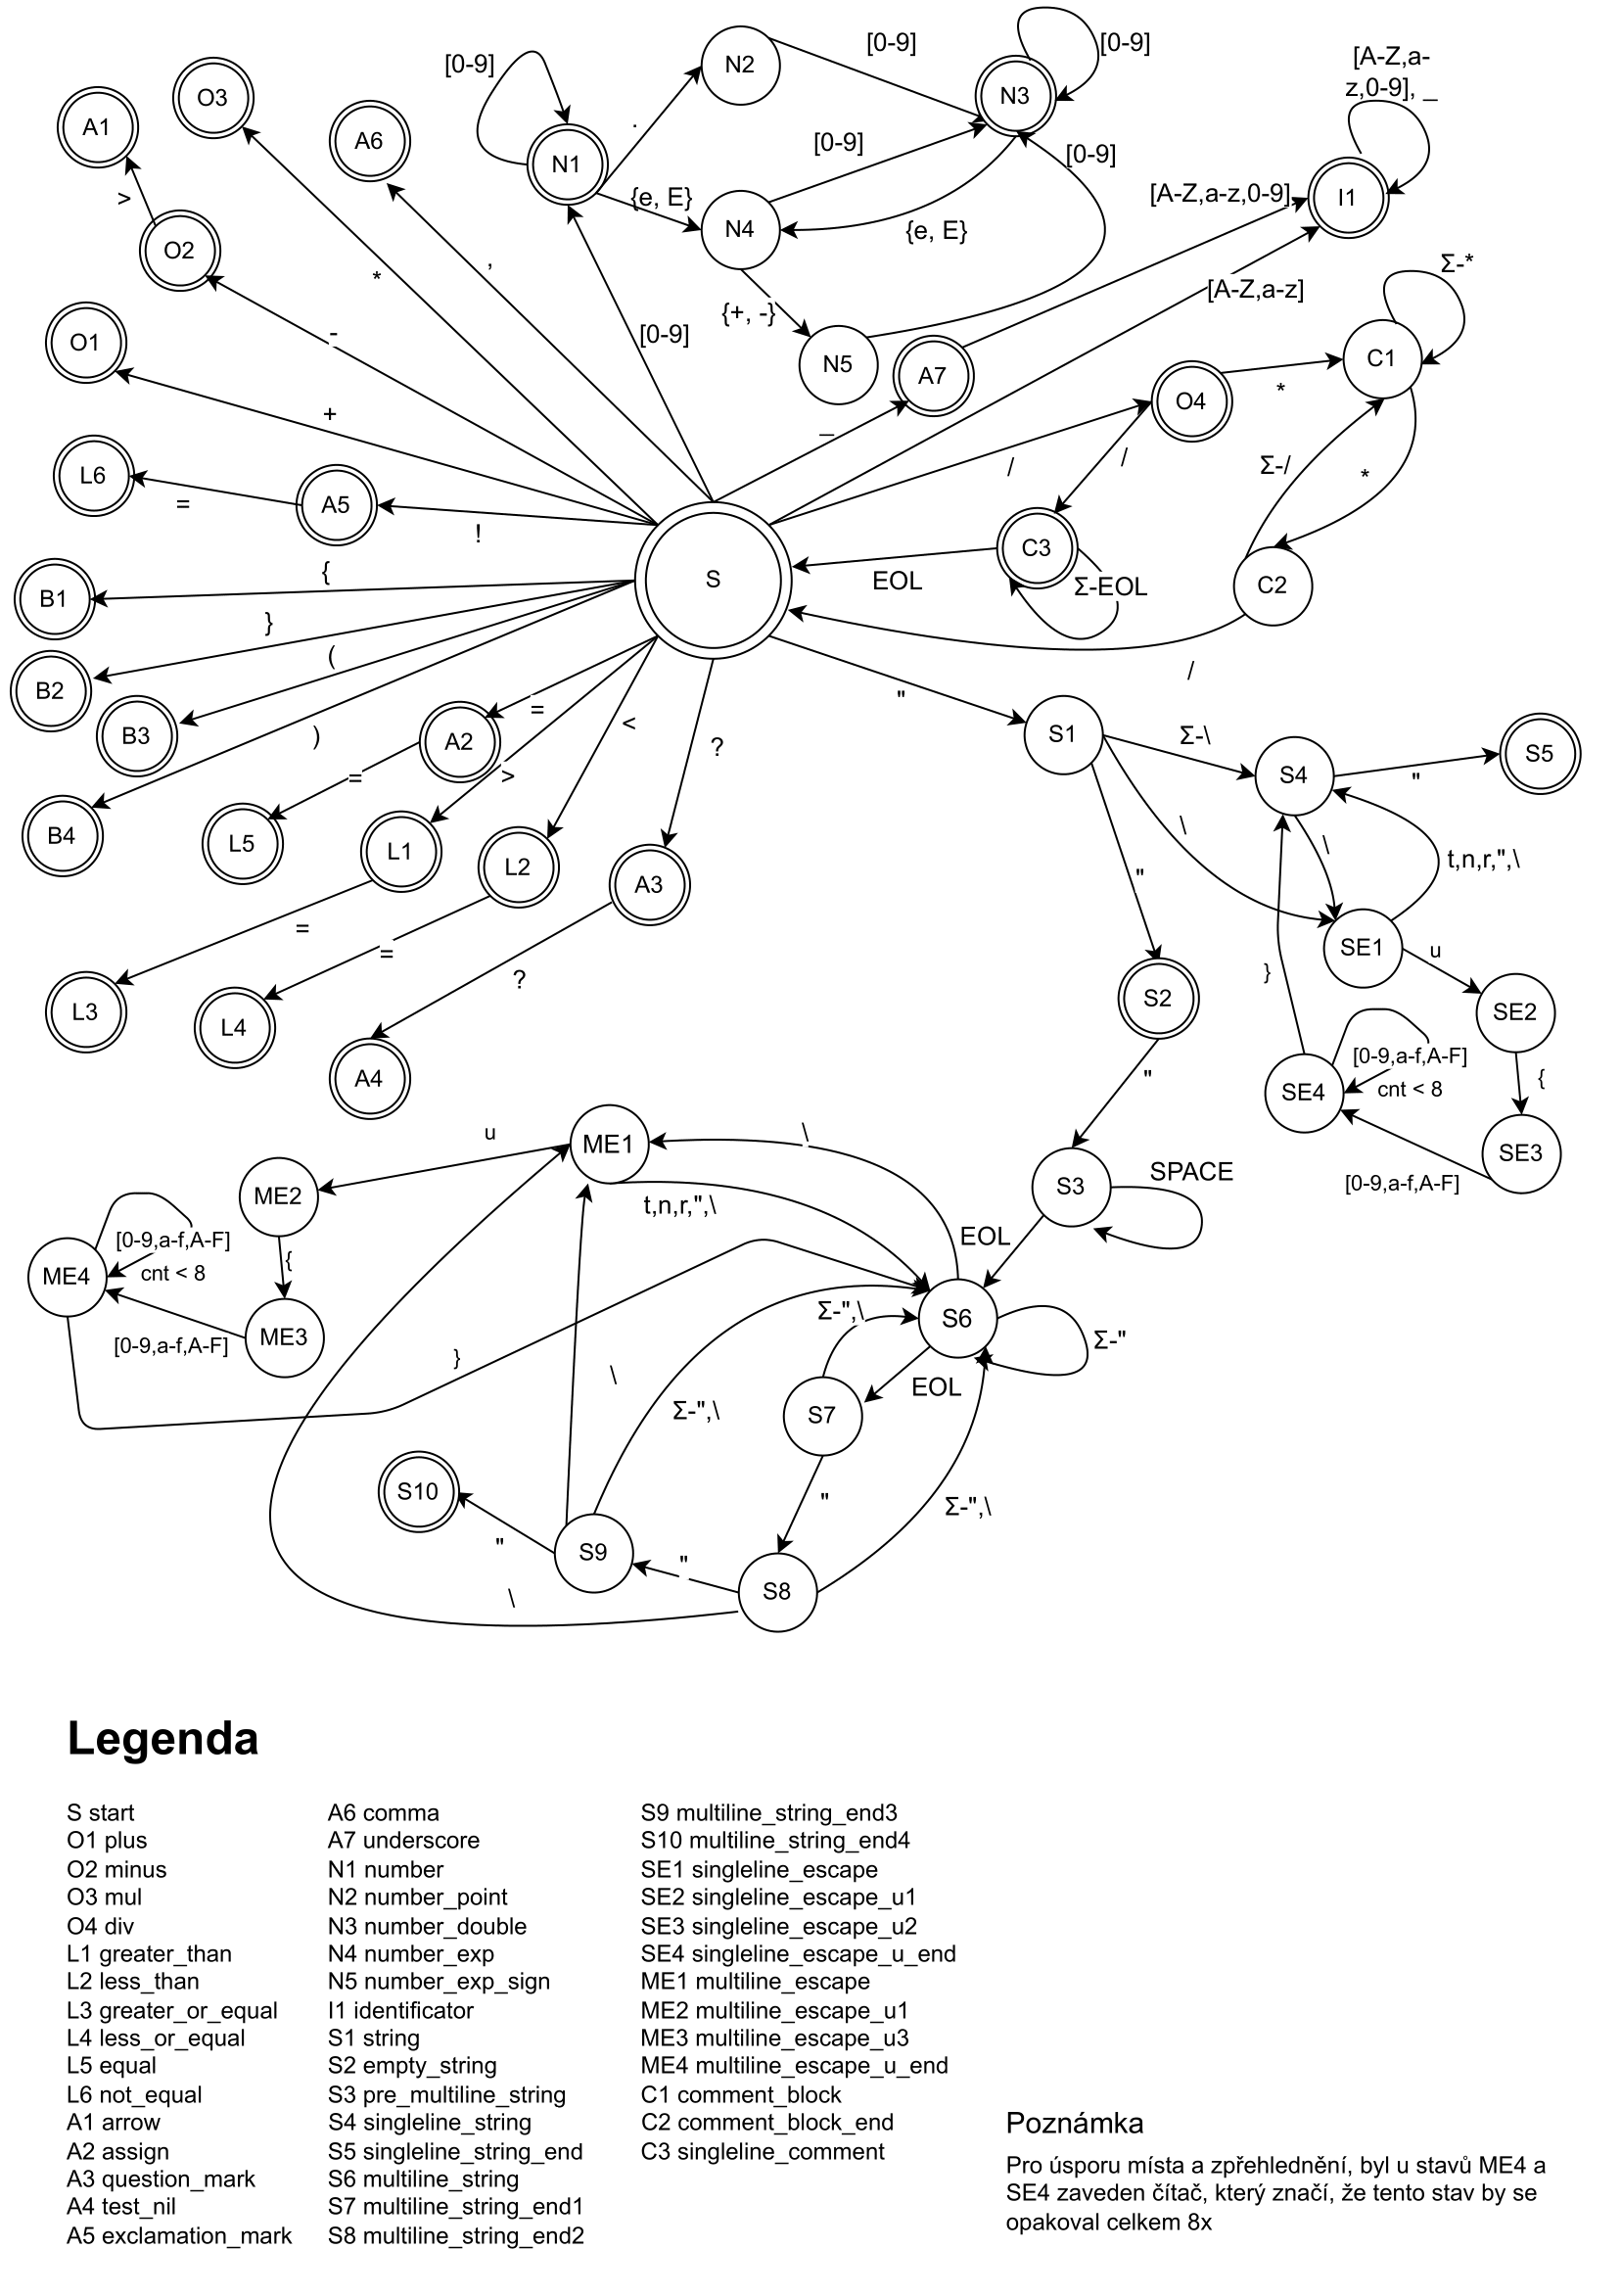
\includegraphics[scale=0.75]{FSM.eps}
\end{figure}

\end{document}